% !TEX encoding = UTF-8
% !TEX TS-program = pdflatex
% !TEX root = ../tesi.tex
% !TEX spellcheck = it-IT

%**************************************************************
\chapter{Analisi dei requisiti}
\label{cap:analisi-requisiti}
%**************************************************************

\intro{Breve introduzione al capitolo}\\

\section{Casi d'uso}

Per lo studio dei casi d'uso del prodotto sono stati realizzati dei diagrammi.
I diagrammi dei casi d'uso (in inglese \emph{Use Case Diagram}) sono diagrammi di tipo \gls{uml} dedicati alla descrizione delle funzioni o servizi offerti da un sistema, così come sono percepiti e utilizzati dagli attori che interagiscono col sistema stesso.
Per ogni \emph{use case} sono stati inoltre riportati:
\begin{itemize}
	\item Attori Principali
	\item Precondizioni
	\item Descrizione/flusso degli eventi
	\item Postcondizioni
\end{itemize}
Seguono i diagrammi riguardanti l'applicativo lato \emph{tablet}, ovvero quello di cui mi sono occupato di persona.

\begin{figure}[!h] 
    \centering 
    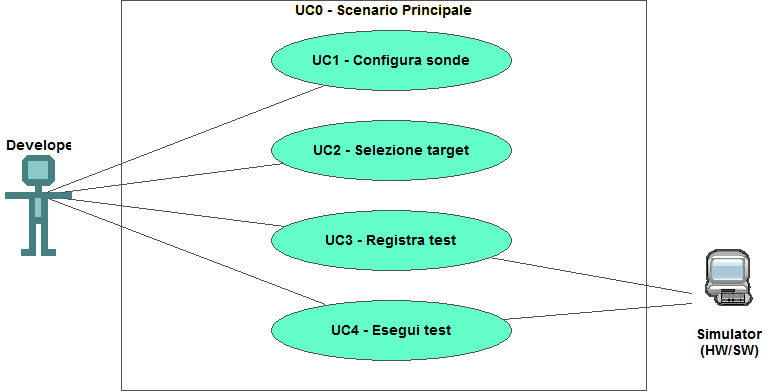
\includegraphics[width=0.9\columnwidth]{usecase/scenario-principale} 
    \caption{Use Case - UC0: Scenario principale}
\end{figure}

\begin{usecase}{0}{Scenario principale}
\usecaseactors{Sviluppatore applicativi}
\usecasepre{Lo sviluppatore è entrato nel plug-in di simulazione all'interno dell'IDE}
\usecasedesc{La finestra di simulazione mette a disposizione i comandi per configurare, registrare o eseguire un test}
\usecasepost{Il sistema è pronto per permettere una nuova interazione}
\label{uc:scenario-principale}
\end{usecase}


\subsection{UC0: Scenario principale}
\begin{figure}[!h] 
    \centering 
    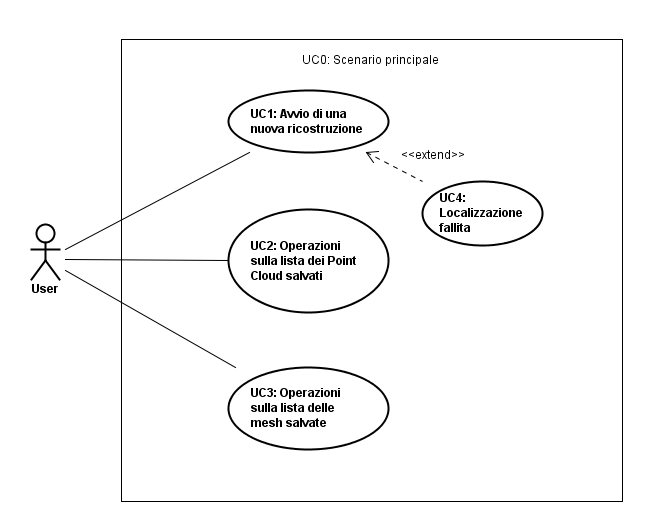
\includegraphics[width=0.9\columnwidth]{usecase/UC0.png} 
    \caption{Use Case - UC0: Scenario principale}
\end{figure}
\ \\
\textbf{Attori Principali}: Utente.
\\\\ \textbf{Precondizioni}: L'utente ha avviato l'applicazione su un dispositivo \emph{Tango} ed ha fornito tutti i permessi necessari, ovvero:
\begin{itemize}
	\item Area Learning (permsso speciale per dispositivi \emph{Tango}.
	\item Lettura e scrittura su disco.
	\item Utilizzo fotocamera.
	\item Accesso ad internet.
\end{itemize}
Inoltente deve aver avviato l'applicazione in un ambiente sufficientemente illuminato.
\\\\ \textbf{Descrizione}: La schermata principale, mentre è immediatamente in atto il processo di localizzazione, mette a disposizione il \emph{render} dei punti e tutti gli strumenti per permettere all'utente effettuare la rilevazione e di accedere agli altri menù.
\\\\ \textbf{Postcondizioni}: Il sistema è pronto per permettere una nuova interazione con l'utente.


\subsection{UC1: Avvio di una nuova ricostruzione}
\begin{figure}[!h] 
    \centering 
    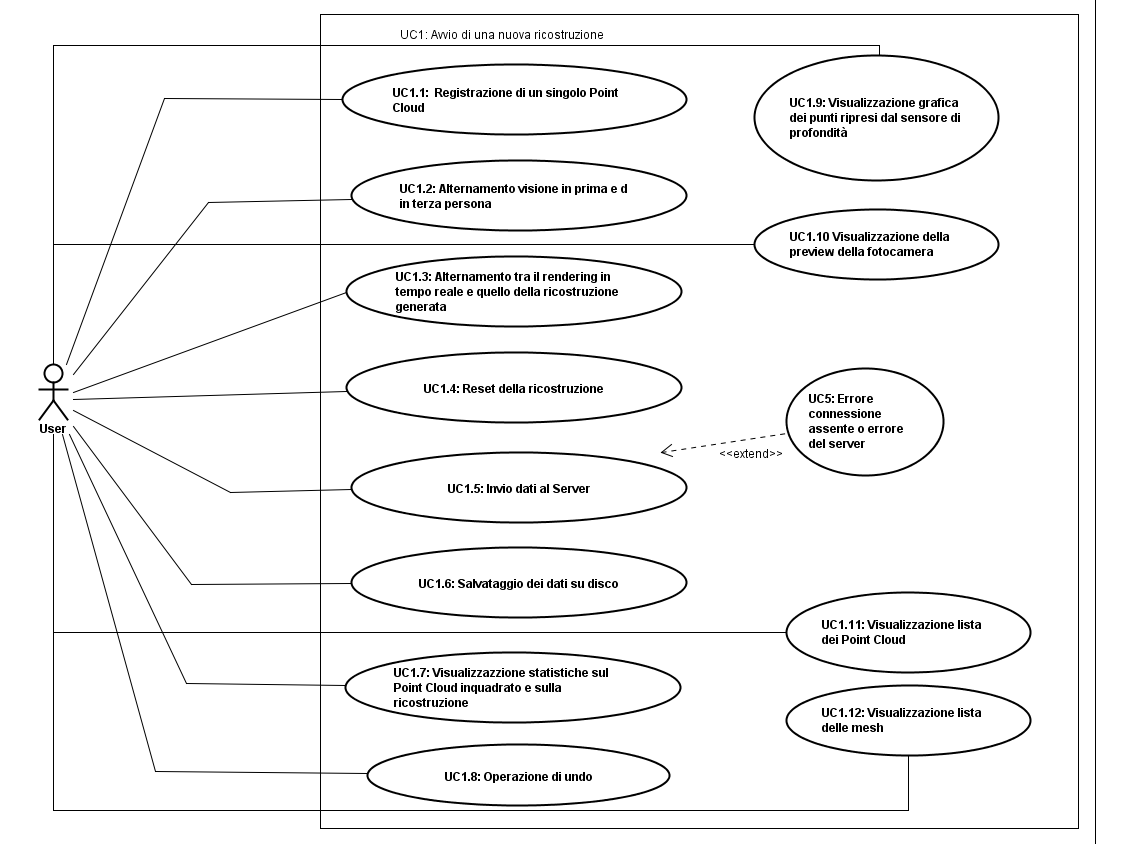
\includegraphics[width=1.0\columnwidth]{usecase/UC1.png} 
    \caption{Use Case - UC1: Avvio di una nuova ricostruzione}
\end{figure}
\ \\
\textbf{Attori Principali}: Utente.
\\\\ \textbf{Precondizioni}: L'utente ha aperto l'applicazione ed è rimasto in attesa della localizzaione nella schermata principale.
\\\\ \textbf{Descrizione}: L'utente ha a disposizione tutti gli strumenti per registrare, controllare e perfezionare la ricostruzione dell'oggetto da inspezionare. Inoltre gli sono forniti i tasti per passare alle altre funzionalità. 
\\\\ \textbf{Postcondizioni}: L'utente ha terminato una registrazione inviandola al \emph{Server}, salvandola su disco, oppure scartandola.



\subsection{UC1.1: Registrazione di un singolo Point Cloud}
\textbf{Attori Principali}: Utente.
\\\\ \textbf{Precondizioni}:  L'utente ha aperto l'applicazione, è rimasto in attesa della localizzaione nella schermata principale ed intende registrare un nuovo scatto.
\\\\ \textbf{Descrizione}: L'utente inquadra il soggetto della rilavazione e preme il tasto "Shot".
\\\\ \textbf{Postcondizioni}: Il sistema ha catturato il \emph{Point Cloud} inquadrato e l'ha aggiunto alla ricostruzione attualmente in corso.

\subsection{UC1.2: Alternamento visione in prima ed in terza persona}
\textbf{Attori Principali}: Utente.
\\\\ \textbf{Precondizioni}: L'utente ha aperto l'applicazione, è rimasto in attesa della localizzaione nella schermata principale e sta osservando il \emph{render}.
\\\\ \textbf{Descrizione}: L'utente, usando i tasti "First" o "Third" alterna tra la visuale in prima ed in terza persona per il \emph{render}.
\\\\ \textbf{Postcondizioni}: Il \emph{render} mostra sullo schermo i suoi contenuti nella modalità scelta dall'utente.

\subsection{UC1.3: Alternamento tra il rendering in tempo reale e quello della ricostruzione generata}
\textbf{Attori Principali}: Utente.
\\\\ \textbf{Precondizioni}: L'utente ha aperto l'applicazione, è rimasto in attesa della localizzaione nella schermata principale ed ha già iniziato la rilevazione, avendo quindi salvato in memoria almeno un Point Cloud singolo.
\\\\ \textbf{Descrizione}: L'utente, usando l'interruttore denominato "Reconstrucion Mode", alterna tra la visualizzazione dei punti attualmente catturati dal sensore di profondità e quella della ricostruzione in corso.
\\\\ \textbf{Postcondizioni}: Il \emph{render} mostra sullo schermo i contenuti selezionati dall'utente.

\subsection{UC1.4: Reset della ricostruzione}
\textbf{Attori Principali}: Utente.
\\\\ \textbf{Precondizioni}: L'utente ha aperto l'applicazione, è rimasto in attesa della localizzaione nella schermata principale ed ha intenzione di scartare interamente la rilevazione effettuata fino a quel momento.
\\\\ \textbf{Descrizione}: L'utente premendo sul pulsante "Reset" azzera i punti salvati e rende il dispositivo pronto per una nuova rilevazione.
\\\\ \textbf{Postcondizioni}: Il dispositivo non ha più alcuna ricostruzione in corso ed è pronto ad iniziarne una nuova.

\subsection{UC1.5: Invio dati al Server}
\textbf{Attori Principali}: Utente.
\\\\ \textbf{Precondizioni}: L'utente ha aperto l'applicazione, è rimasto in attesa della localizzaione nella schermata principale, ha effettuato una rilevazione che lo soddisfa ed intende inviarla al \emph{Server}.
\\\\ \textbf{Descrizione}: L'utente premendo sul pulsante "Send Data To Server" invia la ricostruzione corrente al \emph{Server} in formato \texttt{pcd}.
\\\\ \textbf{Postcondizioni}: La ricostruzione corrente è stata inviata al \emph{Server}, ma non eliminata dalla memoria. Sarà quindi possibile continuare la rilevazione.

\subsection{UC1.6: Salvataggio dei dati su disco}
\textbf{Attori Principali}: Utente.
\\\\ \textbf{Precondizioni}: L'utente ha aperto l'applicazione, è rimasto in attesa della localizzaione nella schermata principale, ha effettuato una rilevazione che lo soddisfa ed intende salvarla su disco.
\\\\ \textbf{Descrizione}: L'utente, premendo sul pulsante "Save" ed inserendo un nome per il \emph{file}, salva la ricostruzione corrente su disco in formato \texttt{pcd}.
\\\\ \textbf{Postcondizioni}: La ricostruzione corrente è stata salvata su disco, ma non eliminata dalla memoria. Sarà quindi possibile continuare la rilevazione.

\subsection{UC1.7: Visualizzazione statistiche}
\textbf{Attori Principali}: Utente.
\\\\ \textbf{Precondizioni}: L'utente ha aperto l'applicazione, è rimasto in attesa della localizzaione nella schermata principale.
\\\\ \textbf{Descrizione}: L'utente può consultare le statistiche riguardanti il \emph{Point Cloud} inquadrato e la ricostruzione nell'angolo in alto a sinistra dello schermo. Tali satistiche sono:
\begin{itemize}
	\item Numero dei punti attualmente inquadrati.
	\item Distanza media dei punti attualmente inquadrati.
	\item Numero degli scatti presi fino a quel momento.
	\item Numero di punti presenti nella ricostruzione fino a quel momento.
	\item \emph{Frame Of Reference} e \emph{Status} della rilevazione.
	\item Posizione $x$, $y$ e $z$ del dispositivo.
\end{itemize} 
\ \\ \textbf{Postcondizioni}: L'utente ha visualizzato le statistiche.

\subsection{UC1.8: Operazione di undo}
\textbf{Attori Principali}: Utente.
\\\\ \textbf{Precondizioni}: L'utente ha aperto l'applicazione, è rimasto in attesa della localizzaione nella schermata principale, ha effettuato uno o più \emph{shot} che ritiene errati o di bassa qualità ed intende scartarli.
\\\\ \textbf{Descrizione}: L'utente, premendo sul pulsante "Undo", scarta l'ultimo \emph{Point Cloud} registrato.
\\\\ \textbf{Postcondizioni}: L'ultimo \emph{Point Cloud} registrato viene scartato.




\subsection{UC2: Operazioni sulla lista dei Point Cloud salvati}
\begin{figure}[!h] 
    \centering 
    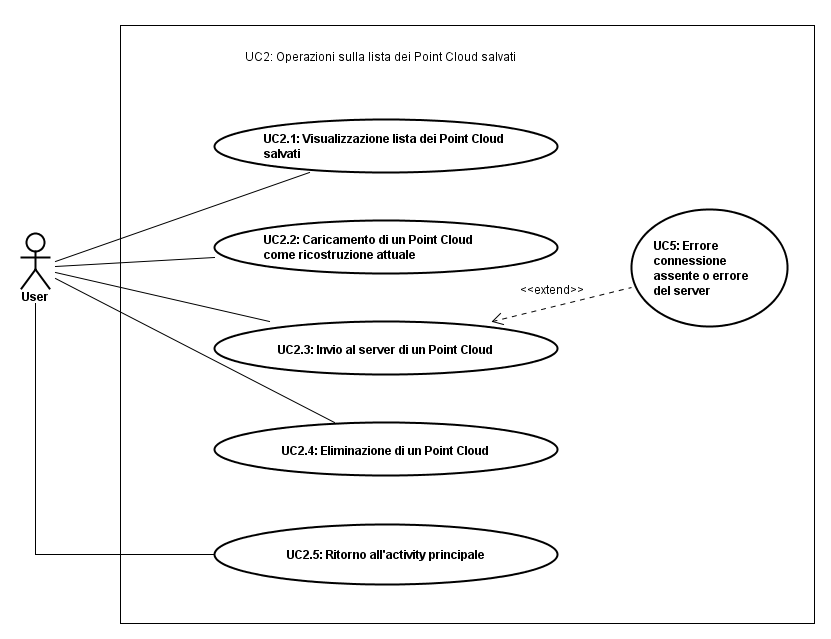
\includegraphics[width=0.9\columnwidth]{usecase/UC2.png} 
    \caption{Use Case - UC2: Operazioni sulla lista dei Point Cloud salvati}
\end{figure}
\ \\
\textbf{Attori Principali}: Utente.
\\\\ \textbf{Precondizioni}: L'utente ha aperto l'applicazione ed ha premuto sul pulsante per visualizzare la lista delle ricostruzioni 3D salvate su disco.
\\\\ \textbf{Descrizione}: L'utente vede sullo schermo la lista delle ricostruzioni 3D salvate su disco su cui può effettuare diverse azioni.
\\\\ \textbf{Postcondizioni}: Il sistema è pronto per ricervere una nuova interazione.


\subsection{UC2.1: Visualizzazione lista dei PointCloud salvati}
\textbf{Attori Principali}: Utente.
\\\\ \textbf{Precondizioni}: L'utente ha aperto l'applicazione, ha premuto sul pulsante per visualizzare la lista delle ricostruzioni 3D salvate su disco.
\\\\ \textbf{Descrizione}: L'utente consulta la lista dei \emph{Point Cloud} salvati su disco.
\\\\ \textbf{Postcondizioni}: Nessuna.

\subsection{UC2.2: Caricamento di un Point Cloud come ricostruzione attuale}
\textbf{Attori Principali}: Utente.
\\\\ \textbf{Precondizioni}: L'utente ha aperto l'applicazione, ha premuto sul pulsante per visualizzare la lista delle ricostruzioni 3D salvate su disco ed intende caricare una di queste come ricostruzione attuale.
\\\\ \textbf{Descrizione}: L'utente, premendo sul nome del \emph{file} scelto, lo carica come ricostruzione corrente.
\\\\ \textbf{Postcondizioni}: Il sistema ritorna all'\emph{activity} principale (quella degli UC1.*) con la ricostruzione caricata da file come ricostruzione corrente.

\subsection{UC2.3: Invio al Server di un Point Cloud}
\textbf{Attori Principali}: Utente.
\\\\ \textbf{Precondizioni}: L'utente ha aperto l'applicazione, ha premuto sul pulsante per visualizzare la lista delle ricostruzioni 3D salvate su disco ed ha intenzione di inviare al server uno dei \emph{Point Cloud} salvati.
\\\\ \textbf{Descrizione}: L'utente applica una lunga pressione sul nome del \emph{file} scelto, apparirà un menù; da quest'ultimo l'utente seleziona "Send To Server" e la ricostruzione sarà mandata al \emph{Server} in formato \texttt{pcd}. Generalemente questa funzione viene sfruttata se quando si effettua una rilevazione non si ha immediatamente la possibilità di inviare i dati tramite \emph{Internet}.
\\\\ \textbf{Postcondizioni}: Il \emph{File} selezionato viene correttamente spedito al \emph{Server}.

\subsection{UC2.4: Eliminazione di un Point Cloud}
\textbf{Attori Principali}: Utente.
\\\\ \textbf{Precondizioni}: L'utente ha aperto l'applicazione, ha premuto sul pulsante per visualizzare la lista delle ricostruzioni 3D salvate su disco ed ha intenzione di cancellare uno dei \emph{File} salvati.
\\\\ \textbf{Descrizione}: L'utente applica una lunga pressione sul nome del \emph{file} scelto, apparirà un menù; da quest'ultimo l'utente seleziona "Delete" ed il \emph{File} selezionato viene cancellato.
\\\\ \textbf{Postcondizioni}: Il \emph{File} selezionato è stato cancellato e non è più presente su disco.

\subsection{UC2.5: Ritorno all'activity principale}
\textbf{Attori Principali}: Utente.
\\\\ \textbf{Precondizioni}: L'utente ha aperto l'applicazione, ha premuto sul pulsante per visualizzare la lista delle ricostruzioni 3D salvate su disco ma desidera ritornare all'\emph{activity} principale.
\\\\ \textbf{Descrizione}: L'utente preme sul tasto "Back" e ritorna all'\emph{activity} principale.
\\\\ \textbf{Postcondizioni}: L'utente ritorna all'\emph{activity} principale.


\subsection{UC3: Operazioni sulla lista delle mesh salvate}
\begin{figure}[!h] 
    \centering 
    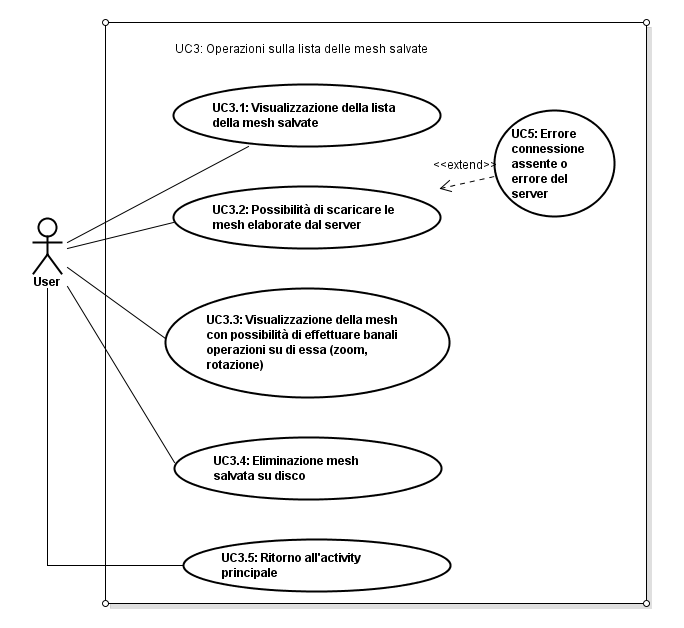
\includegraphics[width=0.9\columnwidth]{usecase/UC3.png} 
    \caption{Use Case - UC3: Operazioni sulla lista delle mesh salvate}
\end{figure}
\ \\
\textbf{Attori Principali}: Utente.
\\\\ \textbf{Precondizioni}: L'utente ha aperto l'applicazione ed ha premuto sul pulsante per visualizzare la lista delle \emph{mesh} salvate su disco.
\\\\ \textbf{Descrizione}: L'utente vede sullo schermo la lista \emph{mesh} salvate su disco su cui può effettuare diverse azioni.
\\\\ \textbf{Postcondizioni}: Il sistema è pronto per ricervere una nuova interazione.




\subsection{UC3.1: Visualizzazione della lista delle mesh salvate}
\textbf{Attori Principali}: Utente.
\\\\ \textbf{Precondizioni}: L'utente ha aperto l'applicazione ed ha premuto sul pulsante per visualizzare la lista delle \emph{mesh} salvate su disco.
\\\\ \textbf{Descrizione}:  L'utente consulta la lista delle \emph{mesh} salvate su disco.
\\\\ \textbf{Postcondizioni}: Nessuna.

\subsection{UC3.2: Possibilità di scaricare le mesh elaborate dal Server}
\textbf{Attori Principali}: Utente.
\\\\ \textbf{Precondizioni}: L'utente ha aperto l'applicazione, ha premuto sul pulsante per visualizzare la lista delle \emph{mesh} salvate su disco ed ha intenzione di aggiornare la lista di \emph{mesh} aggiungendo le altre presenti sul \emph{Server}.
\\\\ \textbf{Descrizione}: L'utente preme sul simbolo di \emph{refresh} in alto a destra e ricarca la lista di \emph{mesh} eventualmente scaricando quelle sul \emph{Server} ma non sul dispositivo.
\\\\ \textbf{Postcondizioni}: L'utente ha a disposizione una lista aggiornata di \emph{mesh}.

\subsection{UC3.3: Visualizzazione grafica delle mesh}
\textbf{Attori Principali}: Utente.
\\\\ \textbf{Precondizioni}: L'utente ha aperto l'applicazione, ha premuto sul pulsante per visualizzare la lista delle \emph{mesh} salvate su disco ed intende visualizzare una specifica \emph{mesh} in 3D.
\\\\ \textbf{Descrizione}: L'utente preme sul nome della \emph{mesh} che intende visualizzare, a questo punto si apre un piccolo ambiente grafico 3D dove l'utente può osservare la ricostruzione ed effettuare banali operazioni di essa.
\\\\ \textbf{Postcondizioni}: Nessuna.

\subsection{UC3.4: Eliminazione mesh salvata su disco}
\textbf{Attori Principali}: Utente.
\\\\ \textbf{Precondizioni}: L'utente ha aperto l'applicazione, ha premuto sul pulsante per visualizzare la lista delle \emph{mesh} salvate su disco.
\\\\ \textbf{Descrizione}: L'utente effettuerà le operazioni necessare per cancellare la \emph{mesh}.
\\\\ \textbf{Postcondizioni}: Il \emph{File} selezionato è stato cancellato e non è più presente su disco.

\subsection{UC3.5: Ritorno all'activity principale}
\textbf{Attori Principali}: Utente.
\\\\ \textbf{Precondizioni}: L'utente ha aperto l'applicazione, ha premuto sul pulsante per visualizzare la lista delle \emph{mesh} salvate su disco ma desidera ritornare all'\emph{activity} principale.
\\\\ \textbf{Descrizione}: L'utente preme sul tasto "Back" e ritorna all'\emph{activity} principale.
\\\\ \textbf{Postcondizioni}: L'utente ritorna all'\emph{activity} principale.


\subsection{UC4: Localizzazione fallita}
\textbf{Attori Principali}: Utente.
\\\\ \textbf{Precondizioni}: Le operazioni di localizzazione non sono andate a buon fine.
\\\\ \textbf{Descrizione}: L'utente non sarà in grado di procedere alla rilevazione, sarà mostrato un messaggio d'errore.
\\\\ \textbf{Postcondizioni}: Non può essere effettuata alcuna rilevazione.


\subsection{UC5: Errore connessione assente o errore del Server}
\textbf{Attori Principali}: Utente.
\\\\ \textbf{Precondizioni}: L'utente cerca di compiere una operazione che richieda comunicazione con il \emph{Server}.
\\\\ \textbf{Descrizione}: L'utente sarà avvisato del fallimento dell'operazione ma potrà ritentare in seguito.
\\\\ \textbf{Postcondizioni}: La comunicazione tra dispositivo e \emph{Server} non va a buon fine.



\section{Requisiti}

Da un'attenta analisi dei requisiti e degli use case effettuata sul progetto è stata stilata la tabella che traccia i requisiti in rapporto agli use case.\\
Sono stati individuati diversi tipi di requisiti e si è quindi fatto utilizzo di un codice identificativo per distinguerli.\\
Il codice dei requisiti è così strutturato R(F/Q/V)(N/D/O) dove:
\begin{enumerate}
	\item[R =] requisito
    \item[F =] funzionale
    \item[Q =] qualitativo
    \item[V =] di vincolo
    \item[N =] obbligatorio (necessario)
    \item[D =] desiderabile
    \item[Z =] opzionale
\end{enumerate}
Nelle tabelle \ref{tab:requisiti-funzionali}, \ref{tab:requisiti-qualitativi} e \ref{tab:requisiti-vincolo} sono riassunti i requisiti e il loro tracciamento con gli use case delineati in fase di analisi.

\newpage

\begin{table}%
\caption{Tabella del tracciamento dei requisti funzionali}
\label{tab:requisiti-funzionali}
\begin{tabularx}{\textwidth}{lXl}
\hline\hline
\textbf{Requisito} & \textbf{Descrizione} & \textbf{Fonti}\\
\hline
RFN-1     & L'interfaccia permette di configurare il tipo di sonde del test & UC1 \\
\hline
\end{tabularx}
\end{table}%

\begin{table}%
\caption{Tabella del tracciamento dei requisiti qualitativi}
\label{tab:requisiti-qualitativi}
\begin{tabularx}{\textwidth}{lXl}
\hline\hline
\textbf{Requisito} & \textbf{Descrizione} & \textbf{Fonti}\\
\hline
RQD-1    & Le prestazioni del simulatore hardware deve garantire la giusta esecuzione dei test e non la generazione di falsi negativi & - \\
\hline
\end{tabularx}
\end{table}%

\begin{table}%
\caption{Tabella del tracciamento dei requisiti di vincolo}
\label{tab:requisiti-vincolo}
\begin{tabularx}{\textwidth}{lXl}
\hline\hline
\textbf{Requisito} & \textbf{Descrizione} & \textbf{Fonti}\\
\hline
RVO-1    & La libreria per l'esecuzione dei test automatici deve essere riutilizzabile & - \\
\hline
\end{tabularx}
\end{table}%